\section{Apresentação}

\begin{frame} % Capa
    \titlepage
\end{frame}

\begin{frame}{Apresentação}
    \begin{itemize}
        \item Professor {\fontfamily{augie}\selectfont Rodrigo de Farias Gomes}
        \item Telefone (somente mensagens): (92) 9 9405-1724
        \item E-mail: shpnft@gmail.com

    \end{itemize}

    \centering

    \vspace{2cm}
    \begin{tabular}{cccccc}
        R & G & O & M & E & S \\ \\
        \(\color{red} \left.\phantom{{\scriptstyle +1}\frac{1}{2}}\right\downarrow {\scriptstyle +1}~~\) &
        \(\color{red} \left.\phantom{{\scriptstyle +1}\frac{1}{2}}\right\downarrow {\scriptstyle +1}~~\) &
        \(\color{red} \left.\phantom{{\scriptstyle +1}\frac{1}{2}}\right\downarrow {\scriptstyle +1}~~\) &
        \(\color{red} \left.\phantom{{\scriptstyle +1}\frac{1}{2}}\right\downarrow {\scriptstyle +1}~~\) &
        \(\color{red} \left.\phantom{{\scriptstyle +1}\frac{1}{2}}\right\downarrow {\scriptstyle +1}~~\) &
        \(\color{red} \left.\phantom{{\scriptstyle +1}\frac{1}{2}}\right\downarrow {\scriptstyle +1}~~\) \\ \\
        S & H & P & N & F & T
    \end{tabular}
\end{frame}

\begin{frame}{Calendário}
    \centering
    \small{
        \begin{tabular}{cP{2cm}P{2cm}P{2cm}P{2cm}P{2cm}}
            \rowcolor{black!10} & Segunda & Terça & Quarta & Quinta & Sexta \\
            01 & \dma{0} & \dma{1} & \dma{2} & \dma{3} & \dma{4} \\
            02 & \dma{7} & \dma{8} & \dma{9} & \dma{10} & \dma{11} \\
            03 & \dma{14} & \dma{15} & \dma{16} & \dma{17} & \dma{18} \\
            04 & \dma{21} & \dma{22} & \dma{23} & \dma{24} & \dma{25} \\
            05 & \dma{28} & \dma{29} & \dma{30} & \dma{31} & \dma{32} \\
            06 & \dma{35} & \dma{36} & \dma{37} & \dma{38} & \dma{39} \\
            07 & \dma{42} & \dma{43} & \dma{44} & \dma{45} & \dma{46} \\
            08 & \dma{49} & \dma{50} & \dma{51} & \dma{52} & \dma{53} \\
            09 & \dma{56} & \dma{57} & \dma{58} & \dma{59} & \dma{60} \\
            10 & \dma{63} & \dma{64} & \dma{65} & \dma{66} & \dma{67} \\
            11 & \dma{70} & \dma{71} & \dma{72} & \dma{73} & \dma{74} \\
            12 & \dma{77} & \dma{78} & \dma{79} & \dma{80} & \dma{81} \\
            13 & \dma{84} & \dma{85} & \dma{86} & \dma{87} & \dma{88} \\
            14 & \dma{91} & \dma{92} & \dma{93} & \dma{94} & \dma{95} \\
            15 & \dma{98} & \dma{99} & \dma{100} & \dma{101} & \dma{102} \\
            % 16 & \dma{103} & \dma{104} & \dma{105} & \dma{106} & \dma{107} \\
            % 17 & \dma{108} & \dma{109} & \dma{110} & \dma{111} & \dma{112} \\
        \end{tabular}
    }
\end{frame}

\begin{frame}{Meus horários em 20/03/2023...}
    \small{
        \begin{center}
            \begin{tabular}{ccccc}
                \rowcolor{black!10} Segunda & Terça & Quarta & Quinta & Sexta \\ \hline
                \rowcolor{red!25} &&&& \\ \hline
                \rowcolor{red!25} Métodos Num... & Trigonometria & Métodos Num... & Trigonometria & \\ \hline
                \rowcolor{green!25} & & Termodinâmica & & Termodinâmica \\ \hline
                \rowcolor{green!25} & Óptica e Eletro... & & Óptica e Eletro... & \\ \hline
                \rowcolor{blue!25} &&&& \\ \hline
                \rowcolor{blue!25} &&&& \\ \hline
            \end{tabular}
        \end{center}

        \vspace{1cm}
        Legenda:
        \begin{itemize}
            \item[\textcolor{red!25}{\rule{1em}{1em}}] Manhã (8:00 -- 10:00 e 10:00 -- 12:00)
            \item[\textcolor{green!25}{\rule{1em}{1em}}] Tarde (14:00 -- 16:00 e 16:00 -- 18:00)
            \item[\textcolor{blue!25}{\rule{1em}{1em}}] Noite (18:00 -- 20:00 e 20:00 -- 22:00)
        \end{itemize}
    }
\end{frame}

\begin{frame}{Ementa de \Disciplina}
    \begin{itemize}
        \item Erros e Sistemas de Numeração
        \item Solução de equações algébricas e transcendentais
        \item Solução de equações polinomiais
        \item Sistemas de equações lineares e não lineares
        \item Interpolação
        \item Ajustamento de curvas
        \item Integração numérica
        \item Solução numérica de equações diferenciais ordinárias e
            sistemas de equações diferenciais
    \end{itemize}
\end{frame}

\begin{frame}{Avaliação}
    \begin{itemize}
        \item A avaliação será na forma de 3 notas: \(N_1\), \(N_2\) e \(N_3\)
        \item A média dos exercícios escolares (\(MEE\)) será dada por
            \[
                MEE=\frac{N_1+N_2+N_3}{3}
            \]
        \item Se \(MEE \geq 8,0\), então a média final (\(MF\)) será igual à \(MEE\)
        \item Se \(MEE < 8,0\), então
            \[
                MF=\frac{2\times MEE+PF}{3}
            \]
            onde PF é a nota da \textbf{prova final}
        \item Se \(MF \geq 5,0\) e a frequência em sala for maior que 75\%, o aluno está aprovado
        \item Haverá 30 aulas de \SI{2}{horas}, de forma que \textbf{o número máximo de faltas é 8}
        % \item Google Sala de Aula:

        %     \centering
        %     https://classroom.google.com/c/NTQzNDU2NTQzODky?cjc=\textcolor{red}{i7z6ybp}
    \end{itemize}
\end{frame}

\begin{frame}{Google Sala de Aula}
    \centering
    \qrcode[height=0.8\textheight]{https://classroom.google.com/c/NTQzNDU2NTQzODky?cjc=i7z6ybp}
    \large{https://classroom.google.com/c/NTQzNDU2NTQzODky?cjc=\textcolor{red}{i7z6ybp}}
\end{frame}

\begin{frame}{Livro texto}
    \centering
    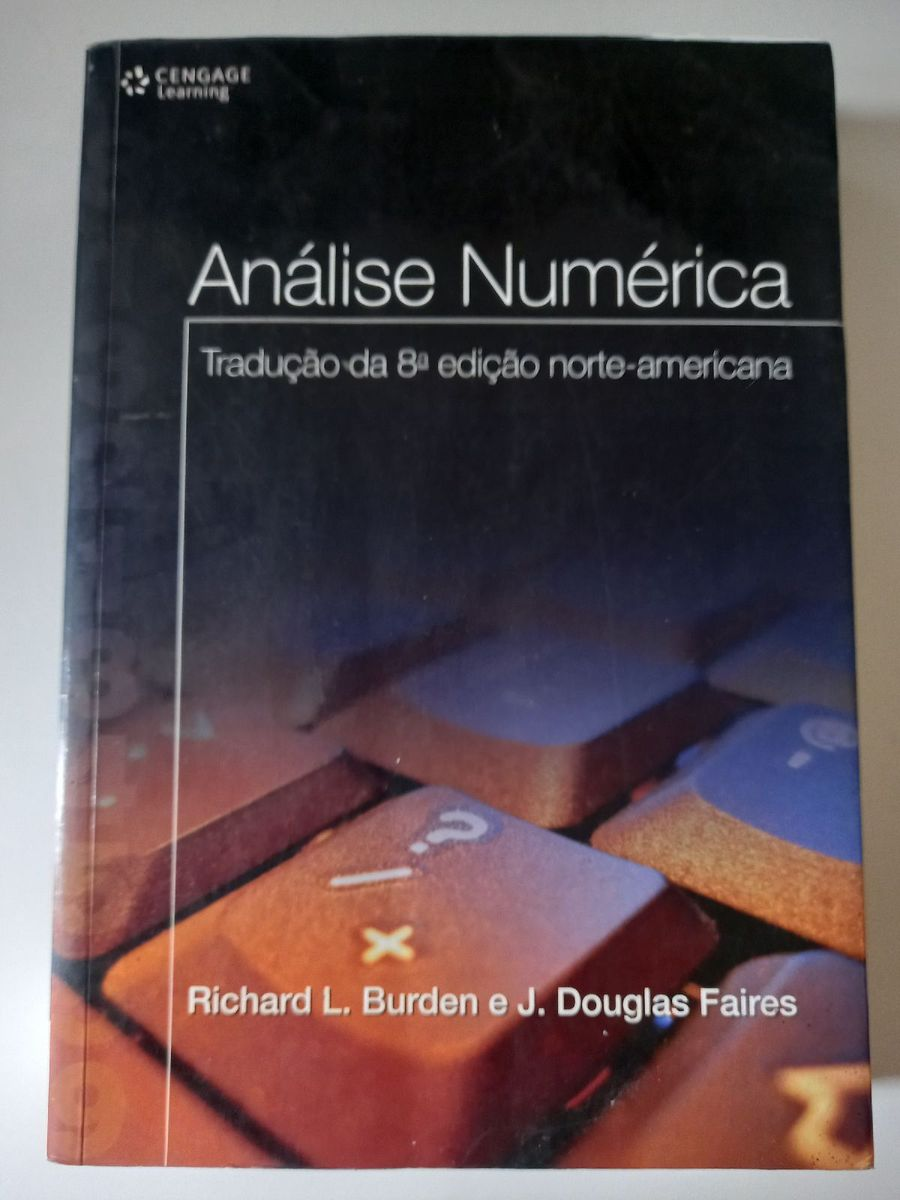
\includegraphics[height=0.8\textheight]{images/livro_burden.jpg}
    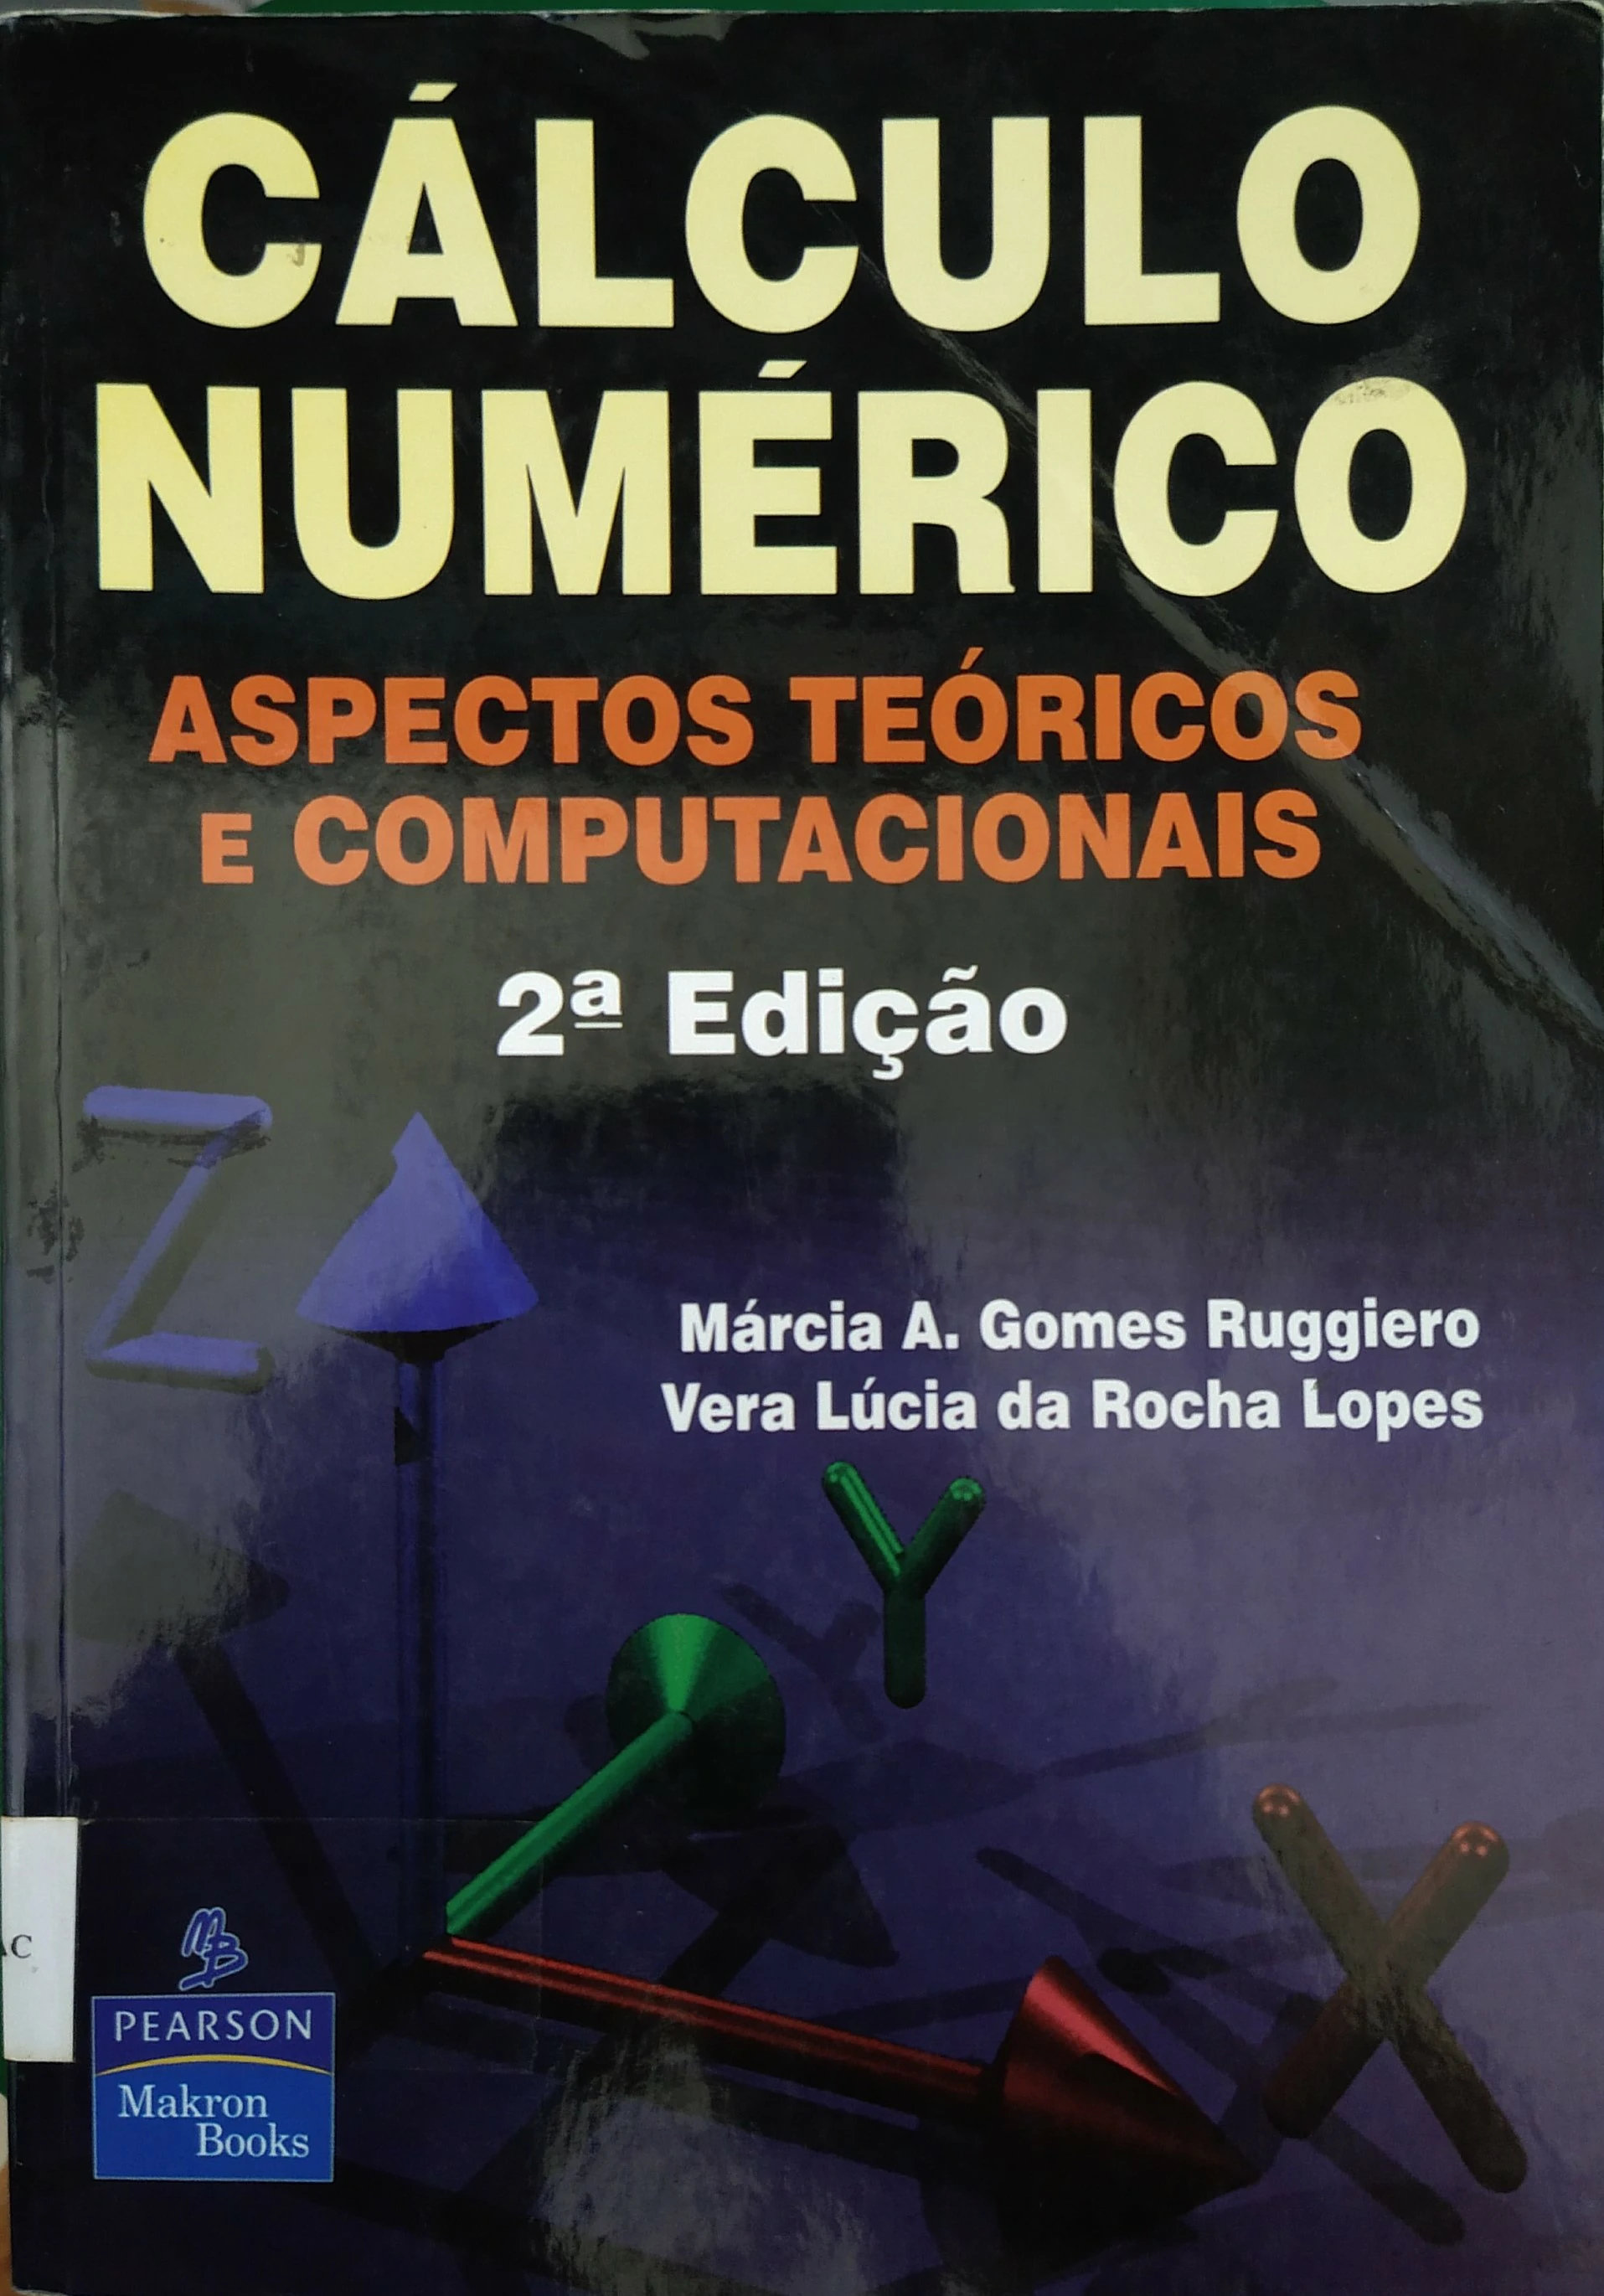
\includegraphics[height=0.8\textheight]{images/ruggiero.png}
\end{frame}

\begin{frame}{Solução analítica}
    \textbf{Soluções analíticas} são baseadas em fórmulas matemáticas em que
    são definidas variáveis de entrada para o cálculo de uma ou mais variáveis
    de saída. Por exemplo, a área de um segmento circular com raio \SI{2.0}{m}
    e profundidade \SI{1.0}{m}

    \begin{center}
        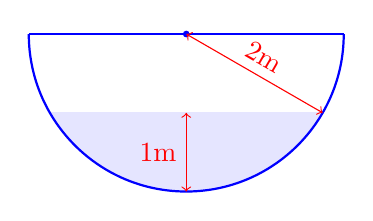
\begin{tikzpicture}[scale=1]
            \begin{scope}
                \clip (-2,-2) -| (2,-1) -| (-2,-2);
                \filldraw [blue!10] (-2,0) arc (180:360:2);
            \end{scope}
            \draw [thick,blue] (-2,0) arc (180:360:2);
            \draw [thick,blue] (-2,0) -- (2,0);
            \filldraw [blue] (0,0) circle (1pt);

            \draw [red, <->] (0,0) -- node [midway,sloped, above] {\SI{2}{m}} +(-30:2);
            \draw [red, <->] (0,-1) -- node [midway,left] {\SI{1}{m}} (0,-2);
        \end{tikzpicture}
    \end{center}
    é dada pela fórmula
    \[
        A=r^2 \arccos{\left(\frac{r-h}{r}\right)}-(r-h)\sqrt{r^2-(r-h)^2} 
        \approx \SI{2.4567}{m^2}
    \]
\end{frame}

\begin{frame}{Métodos numéricos}
    \textbf{Métodos numéricos} são fórmulas ou algoritmos usados para se obter
    \textbf{soluções aproximadas} para um problema matemático que,
    frequentemente, não tem solução analítica. Por exemplo, qual a profundidade
    de um segmento circular com raio \SI{2.0}{m} e área \(\SI{3.0}{m^2}\)?

    \begin{center}
        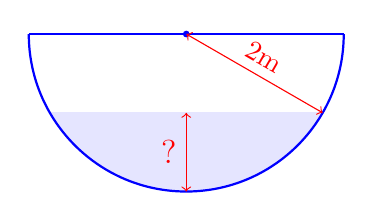
\begin{tikzpicture}[scale=1]
            \begin{scope}
                \clip (-2,-2) -| (2,-1) -| (-2,-2);
                \filldraw [blue!10] (-2,0) arc (180:360:2);
            \end{scope}
            \draw [thick,blue] (-2,0) arc (180:360:2);
            \draw [thick,blue] (-2,0) -- (2,0);
            \filldraw [blue] (0,0) circle (1pt);

            \draw [red, <->] (0,0) -- node [midway,sloped, above] {\SI{2}{m}} +(-30:2);
            \draw [red, <->] (0,-1) -- node [midway,left] {\large{?}} (0,-2);
        \end{tikzpicture}
    \end{center}

    A fórmula para a área é
    \[
        A=r^2 \arccos{\left(\frac{r-h}{r}\right)}-(r-h)\sqrt{r^2-(r-h)^2}
    \]
\end{frame}

\begin{frame}{Método Gráfico}
    \centering
    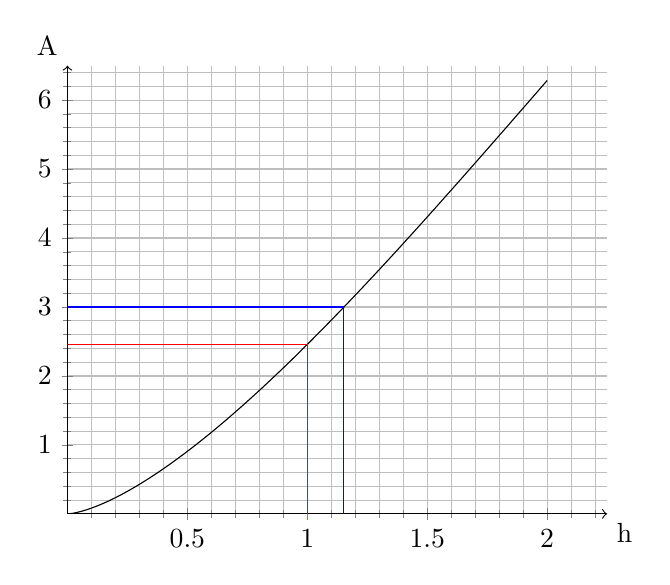
\begin{tikzpicture}
        \begin{axis}[
            axis lines = middle,grid=both,
            axis line style={->},
            minor tick num=4,
            xtick={0,0.5,1,1.5,2,2.5},
            ytick={0,1,2,3,4,5,6,7},
            xmin = 0, xmax=2.25, ymin=0, ymax=6.5,
            x label style={at={(current axis.right of origin)},anchor=north, below right},
            y label style={at={(current axis.above origin)},anchor=south east, above left},
            xlabel={h},
            ylabel={A}
            ]
            \addplot [samples=100, domain=0:2] {2^2 * acos((2-x)/2)*pi/180-(2-x)*sqrt(2^2-(2-x)^2)};
            \draw [red] (axis cs:1,0) |- (axis cs: 0,2.4567);
            \draw [blue] (axis cs:1.15,0) |- (axis cs: 0,3);
        \end{axis}
    \end{tikzpicture}
\end{frame}

\begin{frame}{Método da bissecção}
    \textit{Problema}: Determinar \(x\) tal que \(f(x)=0\)

    \centering
    \begin{tikzpicture}

        \begin{axis}[
            xmin=-3, xmax=3,
            ymin=-10, ymax=10,
            xtick distance=1, ytick distance=4,
            axis x line=center,
            axis y line=center
            ]

            \addplot [domain=-2.5:-2, samples=100, thick, color=red!50] {exp(-x)-x^2};
            \addplot [domain=-2:0.567, samples=100, name path=f1, thick, color=red!50] {exp(-x)-x^2};
            \addplot [domain=0.567:2, samples=100, name path=f2, thick, color=red!50] {exp(-x)-x^2};
            \addplot [domain=2:2.5, samples=100, thick, color=red!50] {exp(-x)-x^2};

            \node[color=red, font=\footnotesize] at (-1.6,4.1) {$f(x)$};

            \only<2>{
                \path [name path=g1] (-3,0) -- (0.567,0);
                \path [name path=g2] (0.567,0) -- (3,0);

                \addplot[blue!20, opacity=0.4] fill between [of=f1 and g1];
                \addplot[red!20, opacity=0.4] fill between [of=f2 and g2];

                \node[color=blue, font=\footnotesize] at (-1.5,1) {$(+)$};
                \node[color=red, font=\footnotesize] at (1.6,-1) {$(-)$};
            }
        \end{axis}

    \end{tikzpicture}
\end{frame}

\begin{frame}{Método da bissecção}
    \textit{Problema}: Determinar \(x\) tal que \(f(x)=0\)

    \centering
    \begin{tikzpicture}

        \begin{axis}[
            xmin=-3, xmax=3,
            ymin=-10, ymax=10,
            xtick distance=1, ytick distance=4,
            axis x line=center,
            axis y line=none
            ]

            \addplot [domain=-2.5:-2, samples=100, thick, color=red!50] {exp(-x)-x^2};
            \addplot [domain=-2:0.567, samples=100, name path=f1, thick, color=red!50] {exp(-x)-x^2};
            \addplot [domain=0.567:2, samples=100, name path=f2, thick, color=red!50] {exp(-x)-x^2};
            \addplot [domain=2:2.5, samples=100, thick, color=red!50] {exp(-x)-x^2};

            \node[color=red, font=\footnotesize] at (-1.6,4.1) {$f(x)$};

            \path [name path=g1] (-3,0) -- (0.567,0);
            \path [name path=g2] (0.567,0) -- (3,0);

            \addplot[blue!20, opacity=0.4] fill between [of=f1 and g1];
            \addplot[red!20, opacity=0.4] fill between [of=f2 and g2];

            \node[color=blue, font=\footnotesize] at (-1.5,1) {$(+)$};
            \node[color=red, font=\footnotesize] at (1.6,-1) {$(-)$};

            \only<2-3>{
                \draw[dashed, black!70, below] (0,-6) node (xr) {$x_r$} -- (0,6) ;
                \draw[dashed, black!70, below] (-2,-6) node (xa) {$x_a$} -- (-2,6) ;
                \draw[dashed, black!70, below] (2,-6) node (xb) {$x_b$} -- (2,6) ;
            }

            \only<3> {
                \draw[->, red] (xa.south) to [out=330,in=-150] (xr.south);
            }

            \only<4-5>{
                \draw[dashed, black!70, below] (1,-6) node (xr) {$x_r$} -- (1,6) ;
                \draw[dashed, black!70, below] (0,-6) node (xa) {$x_a$} -- (0,6) ;
                \draw[dashed, black!70, below] (2,-6) node (xb) {$x_b$} -- (2,6) ;
            }

            \only<5> {
                \draw[->, red] (xb.south) to [out=-150,in=-30] (xr.south);
            }

            \only<6-7>{
                \draw[dashed, black!70, below] (0.5,-6) node (xr) {$x_r$} -- (0.5,6) ;
                \draw[dashed, black!70, below] (0,-6) node (xa) {$x_a$} -- (0,6) ;
                \draw[dashed, black!70, below] (1,-6) node (xb) {$x_b$} -- (1,6) ;
            }

            \only<7> {
                \draw[->, red] (xa.south) to [out=-30,in=-150] (xr.south);
            }

        \end{axis}

    \end{tikzpicture}
\end{frame}

\begin{frame}{Método da bissecção}
    \begin{enumerate}
        \item Reescreve-se o problema de forma que se torne ''Determinar \(x\) tal que \(f(x)=0\)''
        \item Estima-se dois valores, $x_a$ e $x_b$ tal que $f(x_a)$ e $f(x_b)$ tenham sinais diferentes
        \item \label{calculo} Calcula-se o ponto médio \(x_r\) do intervalo formado por $x_a$ e $x_b$:
            \[
                x_r=\frac{x_a + x_b}{2}
            \]
        \item \label{escolha} Se o sinal de $f(x_a)$ é igual ao de $f(x_r)$ , então $x_a = x_r$, senão $x_b=x_r$
        \item Repetimos \ref{calculo} e \ref{escolha} até $f(x_r)=0$ ou \textit{outro critério de parada}
    \end{enumerate}

    \pause
    \begin{tcolorbox}[colback=red!10]
        Atividade: Determine \(h\) tal que
        \[
            A=r^2 \arccos{\left(\frac{r-h}{r}\right)}-(r-h)\sqrt{r^2-(r-h)^2}
        \]
        onde \(A=\SI{3}{m^2}\) e \(r=\SI{2}{m}\)
    \end{tcolorbox}
\end{frame}

\begin{frame}{Tabela}
    \(\rightarrow\) A iteração 0 é onde \textit{escolhemos} o ponto de partida do método

    \centering
    \begin{tabular}{c|P{1.75cm}|P{1.75cm}|P{1.75cm}|P{1.75cm}|P{1.75cm}|P{1.75cm}}
        \(i\) & \(h_a\) & \(h_b\) & \(h_r\) & \(f(h_a)\) & \(f(h_b)\) & \(f(h_r)\) \\ \hline\pause
        0 & 0,00000 & 2,00000 & 1,00000 & 3,00000 & -3,28319 & 0,54326 \\ \hline\pause
        1 & 1,00000 & 2,00000 & 1,50000 & 0,54326 & -3,28319 & -1,30422 \\ \hline\pause
        2 & 1,00000 & 1,50000 & 1,25000 & 0,54326 & -1,30422 & -0,35506 \\ \hline\pause
        3 & 1,00000 & 1,25000 & 1,12500 & 0,54326 & -0,35506 & 0,10171 \\ \hline\pause
        4 & 1,12500 & 1,25000 & 1,18750 & 0,10171 & -0,35506 & -0,12494 \\ \hline\pause
        5 & 1,12500 & 1,18750 & 1,15625 & 0,10171 & -0,12494 & -0,01116 \\ \hline\pause
        6 & 1,12500 & 1,15625 & 1,14063 & 0,10171 & -0,01116 & 0,04539 \\ \hline\pause
        7 & 1,14063 & 1,15625 & 1,14844 & 0,04539 & -0,01116 & 0,01715 \\ \hline\pause
        8 & 1,14844 & 1,15625 & 1,15234 & 0,01715 & -0,01116 & 0,00300 \\ \hline\pause
        9 & 1,15234 & 1,15625 & 1,15430 & 0,00300 & -0,01116 & -0,00408 \\ \hline\pause
        10 & 1,15234 & 1,15430 & 1,15332 & 0,00300 & -0,00408 & -0,00054 \\ \hline\pause
        11 & 1,15234 & 1,15332 & 1,15283 & 0,00300 & -0,00054 & 0,00123 \\ \hline\pause
        12 & 1,15283 & 1,15332 & 1,15308 & 0,00123 & -0,00054 & 0,00035
    \end{tabular}
\end{frame}

\begin{frame}{Tabela (continuação)}
    \begin{center}
        \begin{tabular}{c|P{1.75cm}|P{1.75cm}|P{1.75cm}|P{1.75cm}|P{1.75cm}|P{1.75cm}}
            \(i\) & \(x_a\) & \(x_b\) & \(x_r\) & \(f(x_a)\) & \(f(x_b)\) & \(f(x_r)\) \\ \hline
            13 & 1,15308 & 1,15332 & 1,15320 & 0,00035 & -0,00054 & -0,00009 \\ \hline
            14 & 1,15308 & 1,15320 & 1,15314 & 0,00035 & -0,00009 & 0,00013 \\ \hline
            15 & 1,15314 & 1,15320 & 1,15317 & 0,00013 & -0,00009 & 0,00002 \\ \hline
            16 & 1,15317 & 1,15320 & 1,15318 & 0,00002 & -0,00009 & -0,00004 \\ \hline
            17 & 1,15317 & 1,15318 & 1,15318 & 0,00002 & -0,00004 & -0,00001 \\ \hline
            18 & 1,15317 & 1,15318 & 1,15317 & 0,00002 & -0,00001 & 0,00000 \\ \hline
            19 & 1,15317 & 1,15318 & 1,15317 & 0,00000 & -0,00001 & 0,00000 \\ \hline
            20 & 1,15317 & 1,15317 & 1,15317 & 0,00000 & 0,00000 & 0,00000 \\ \hline
            21 & 1,15317 & 1,15317 & 1,15317 & 0,00000 & 0,00000 & 0,00000 \\ \hline
            22 & 1,15317 & 1,15317 & 1,15317 & 0,00000 & 0,00000 & 0,00000 \\ \hline
            23 & 1,15317 & 1,15317 & 1,15317 & 0,00000 & 0,00000 & 0,00000 \\ \hline
            24 & 1,15317 & 1,15317 & 1,15317 & 0,00000 & 0,00000 & 0,00000 \\ \hline
        \end{tabular}
    \end{center}
\end{frame}

% aula prática
\begin{frame}{A função \textit{SE}}
    \begin{itemize}
        \item A função \textit{SE} ''retorna um valor se uma expressão lógica for verdadeira e outro se for falsa'':
            \begin{center}
                \fbox{\texttt{=SE(expressão\_lógica; valor\_se\_verdadeiro; valor\_se\_falso)}}
                \vspace{1em}
            \end{center}
        \item Assumindo que \(x_a\) está B2, \(x_b\) está C2, \(x_r\) está D2, \(f(x_a)\) está em E2, \(f(x_b)\) está em F2 e \(f(x_r)\) está em G2, a expressão
            \begin{center}
                \fbox{\texttt{=SE(E2*G2>=0; D2; B2)}}
                \vspace{1em}
            \end{center}
            será igual a \(x_r\) se \(f(x_a)\) tiver o mesmo sinal que \(f(x_r)\), caso contrário a expressão será igual a \(x_a\)
    \end{itemize}
\end{frame}

\begin{frame}[label=chant]{Exercícios}
    Determine \(x\) (ou \(h\)) tal que
    \begin{enumerate}
        \item<1> \(r^2 \arccos{\left(\frac{r-h}{r}\right)}-(r-h)\sqrt{r^2-(r-h)^2}=3\) onde \(r=2\)
        \item \(e^{-x}=x\)
        \item \(\ln(x-1) + \cos(x-1)=0 \)
        \item \(e^x=3x^2\)
        \item \((x-2)^2=\ln x\)
    \end{enumerate}
\end{frame}

\begin{frame}{Como armazenar ''números''}
    \begin{itemize}
        \item Um número inteiro (sem casas decimais) pode ser armazenado na forma de um odômetro:
            \begin{center}
                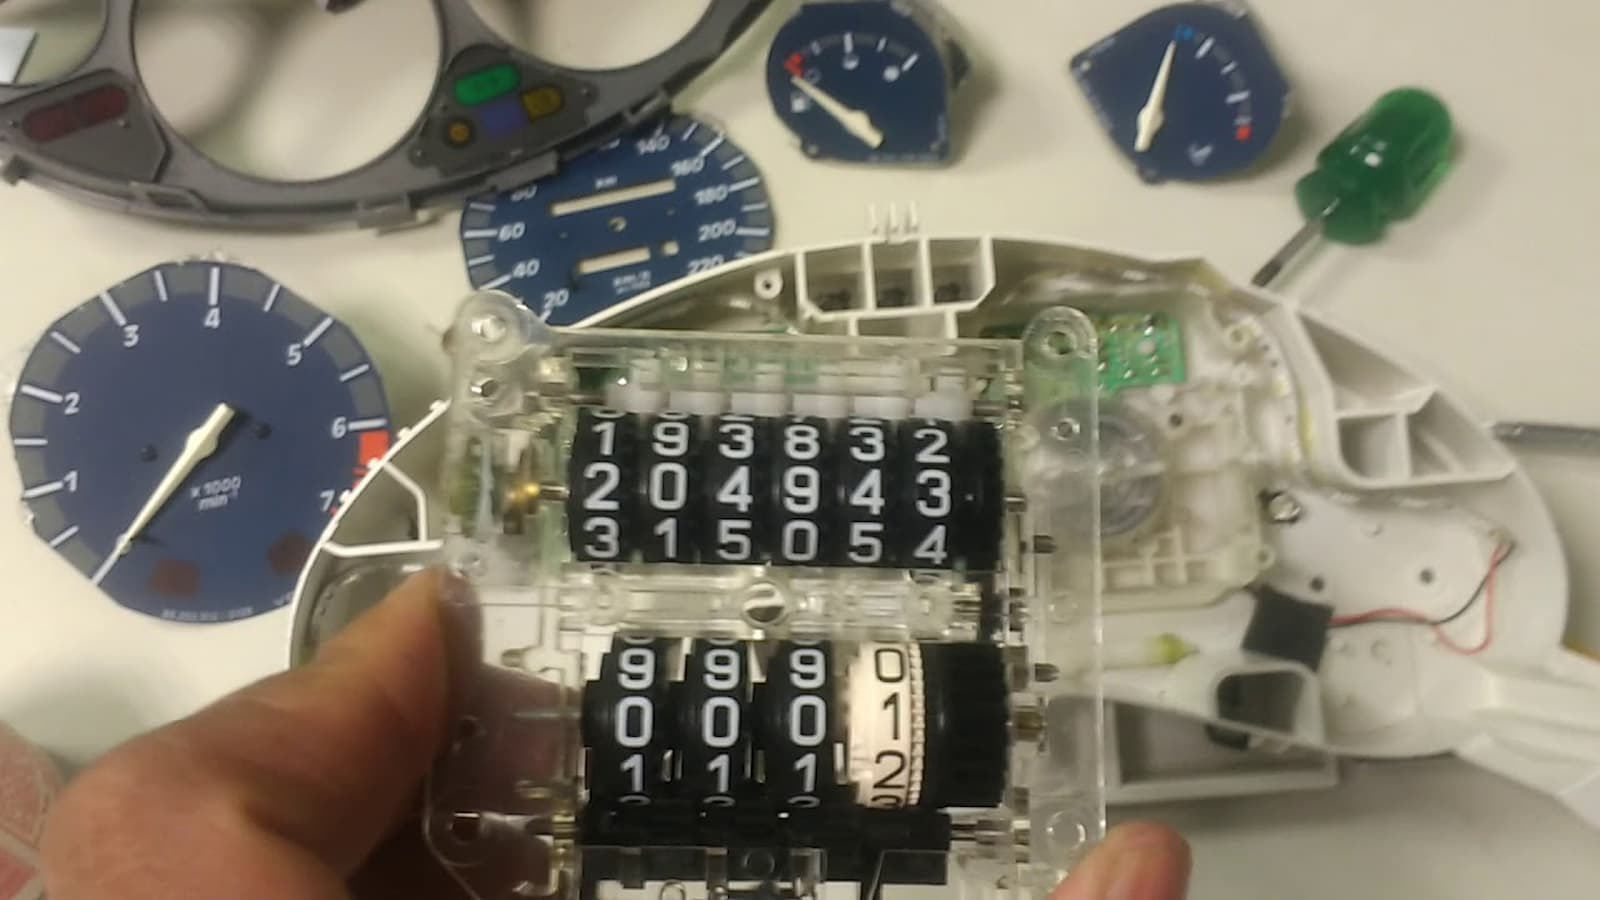
\includegraphics[height=0.5\textheight]{images/odometro.jpg}
            \end{center}
        \item O número de ''dígitos'' depende da construção do odômetro
        \item O intervalo de valores que os ''dígitos'' podem ter depende da construção do odômetro
    \end{itemize}
\end{frame}

\begin{frame}{Exemplo: Relógio}
        Tem 2 dígitos, um pode ir de 0 até 59 e o outro de 1 até 12

            \begin{center}
                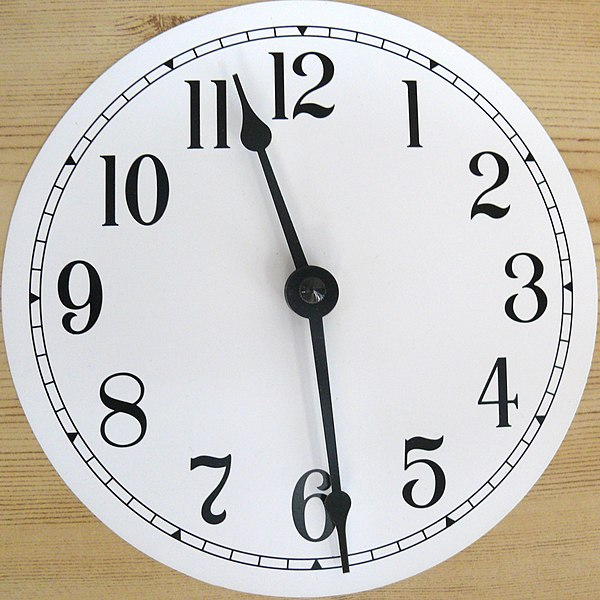
\includegraphics[height=0.65\textheight]{images/clock.jpeg}
            \end{center}
\end{frame}

\begin{frame}{Computadores \textit{modernos}}
    \begin{itemize}
        \item Têm odômetros com números de dígitos múltiplo de 8
        \item Um odômetro com 8 dígitos tem \SI{1}{byte} de tamanho, um odômetro 
            com 16 dígitos tem \SI{2}{bytes} etc
        \item Cada dígito é chamado de \textit{bit} e só pode ser 0 ou 1
        \item  \SI{1}{byte}=\SI{8}{bits}
        \item Qual o maior número que pode ser
            armazenado com \SI{4}{bytes} (padrão na maioria dos sistemas)? 
    \end{itemize}

    \centering
    
\includegraphics[height=0.55\textheight-16.32pt]{images/Captura de tela de 2023-03-26 23-58-54.png}
\end{frame}

\begin{frame}
    \begin{center}
        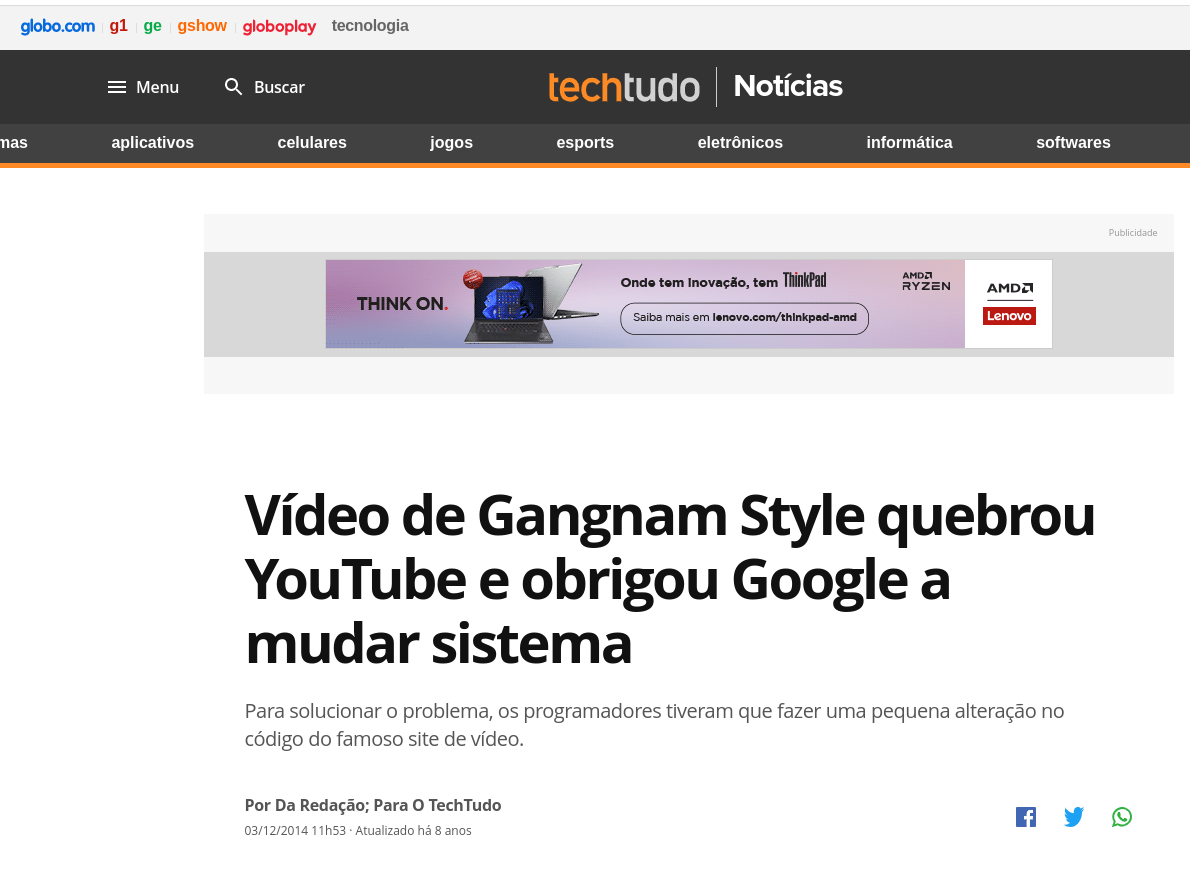
\includegraphics[height=0.9\textheight]{images/Captura de tela de 2023-03-27 00-22-46.png}
    \end{center}
\end{frame}

\begin{frame}[c]
    \frametitle{Conversão de binário para decimal}
    \[
        11001_{2}  = 1 \cdot 2^4 + 1 \cdot 2^3 + 0 \cdot 2^2 + 0 \cdot 2^1 + 1 \cdot 2^0 =25_{10}
    \]
\end{frame}

\begin{frame}{\textit{Extra}: Conversão de decimal para binário}
    \[
        25_{10} = d_1 \cdot 2^4 + d_2 \cdot 2^3 + d_3 \cdot 2^2 + d_4 \cdot 2^1 + d_5 \cdot 2^0 = 
        (d_1 d_2 d_3 d_4 d_5)_{2}
    \]
    \begin{itemize}
        \item Por que \(2^4\) e não \(2^5\)?
        \item Temos que \(d_1 = 25 / 2^4 \) que é igual a 1 \textbf{com resto 9}
        \item Temos que \(d_2 = 9 / 2^3\) que é igual a 1 \textbf{com resto 1}
        \item Temos que \(d_3 = 1 / 2^2\) que é igual a 0 \textbf{com resto 1}
        \item Temos que \(d_4 = 1 / 2^1\) que é igual a 0 \textbf{com resto 1}
        \item Temos que \(d_5 = 1 / 2^0\) que é igual a 1 \textbf{com resto 0} (sempre)
        \item Assim, temos que \(25_{10} = 11001_{2}\)
    \end{itemize}
\end{frame}

\begin{frame}[c]
    \frametitle{\textit{Extra}: Conversão de decimal para binário}
    \begin{center}
        \begin{tikzpicture}
            \coordinate (D-1-2) at (0,0) {}; % We must start with this command.
            \Division{25}{2}{1} % First dividend, divisor, remainder
            \Division{12}{2}{0} % Dividend (previous quotient), divisor, remainder
            \Division{6}{2}{0}  
            \Division{3}{2}{1}  
            \FinDivision{1}     % Last remainder.

            \only<2->{
                % We can draw an arrow jumping from one remainder 
                % to the next one. Every reminder is a node called
                % Rdividend. Last remainder is node C.
                \draw[red,shorten <=1mm, ->, dashed] (C) to[out=-150,in=-65] (R3);
                \draw[red,shorten <=1mm, ->, dashed] (R3) to[out=-150,in=-65] (R6);
                \draw[red,shorten <=1mm, ->, dashed] (R6) to[out=-150,in=-65] (R12);
                \draw[red,shorten <=1mm, ->, dashed] (R12) to[out=-150,in=-65] (R25);
            }
        \end{tikzpicture}

        \only<2->{
            \[
                25_{10} = 11001_{2}
            \]
        }
    \end{center}
\end{frame}

\begin{frame}{Números com casas decimais: aritmética de ponto flutuante}
    \begin{tcolorbox}[colback=red!10]
        Na \textit{aritmética de ponto flutuante}, um número ''com casas decimais'' é representado
        na forma:
        \[
            \pm (0 . d_1 d_2 d_3 \ldots d_k) \times \beta^e
        \]
        onde \(d_ 1 d_2 d_3 \ldots d_k\) é a mantissa, \(\beta\) é a base e \(e\) é o expoente
    \end{tcolorbox}
    \pause
    Na maioria dos sistemas (IEEE-754), temos base 2 com \SI{1}{bit} para sinal e
    \begin{itemize}
        \item \textit{Precisão simples}: \SI{8}{bits} de expoente e \SI{23}{bits} de mantissa, num total de 
            \SI{32}{bits} (\SI{4}{bytes})
        \item \textit{Precisão dupla}: \SI{11}{bits} de expoente e \SI{52}{bits} de mantissa, num total de 
            \SI{64}{bits} (\SI{8}{bytes})
        \item Os expoentes são deslocados pela metade \textit{inteira} do maior
            valor possível (127 ou 1023)
        \item O maior e o menor expoentes possíveis são reservados para \alert{casos especiais}
        \item Os números são \textit{normalizados}: \( \pm (1 . d_1 d_2 d_3 \ldots d_k) \times 2^e\) 
            ao invés de \( \pm (0 . d_1 d_2 d_3 \ldots d_k) \times 2^e\)
    \end{itemize}
    \pause
    \begin{tcolorbox}[colback=blue!10]
        Qual é o maior e o menor número positivo que pode ser representado no padrão IEEE-754, precisão simples?

        \tiny{Resposta: \(0~00000001~0000 0000 0000 0000 0000 000\) e \(0~11111110~1111 1111 1111 11111 111 111\)}
    \end{tcolorbox}
\end{frame}


\begin{frame}
    \frametitle{Método de Newton-Raphson}

    Sendo \(x_0\) uma aproximação inicial (''chute''), podemos obter uma aproximação ''melhor'' através da fórmula
    \begin{block}
        {}
        \[ x_{k+1} = x_k - \frac{f(x_k)}{f'(x_k)} \]
    \end{block}
    onde \(k=0,1,2,\ldots\) é o número da \textbf{iteração}. 

    O método de Newton-Raphson
    \begin{itemize}
        \item É um método \textit{aberto}, isto é, é necessário apenas um valor inicial \(x_0\)
        \item Algumas vezes \textit{diverge}, ou seja, o resultado obtido em cada iteração se afasta da raiz verdadeira
        \item Mas quando há convergência o resultado obtido em cada iteração se aproxima da raiz verdadeira muito mais rápido do que o método da bissecção
    \end{itemize}
\end{frame}

\begin{frame}{Atividade}
    \begin{itemize}
        \item Determine \(x\) tal que \(f(x)=0\) onde
            \[
                \color{blue}
                \boxed{f(x)=x^2+3x-4}
            \]
            usando o método de Newton Raphson com derivada analítica
            \[
                \color{blue}
                \boxed{f'(x)=2x+3}
            \]
    \end{itemize}
\end{frame}

\begin{frame}{Atividade}
    Determine \(h\) tal que

    \[
        \color{blue}
        r^2 \arccos{\left(\frac{r-h}{r}\right)}-(r-h)\sqrt{r^2-(r-h)^2}=3
    \]
    onde \(r=2\) usando o método de Newton Raphson com derivada analítica
    \[
        \color{blue}
        \frac{d}{dx} \left( 
            r^2 \arccos{\left(\frac{r-h}{r}\right)}-(r-h)\sqrt{r^2-(r-h)^2}
        \right)=
        2\sqrt{h(2r-h)}
    \]
\end{frame}

\againframe<2->{chant}

\begin{frame}{Estudo dirigido}
    \begin{itemize}
        \item Converta \num{100.1} e \num{100.5} para o padrão IEEE-754, precisão simples
        \item Qual dos dois números é representado de forma mais ''exata''?
    \end{itemize}
\end{frame}
